\documentclass[11pt]{article}
\usepackage[margin=1in]{geometry}
\usepackage{graphicx}
\usepackage{amsmath}
\usepackage{amssymb}
\usepackage{float}
\usepackage{subcaption}
\usepackage{booktabs}

\title{Busyness Analysis}

\begin{document}
\maketitle

\section{Key Takeaways}
  \begin{itemize}
    \item \textbf{Baseline Service Rate Estimates:} I used a simple linear regression model
    to estimate $\mu_p$ and $\mu_t$. The model seems to fit the data well ($R^2$=0.97) and
    yields estimates of 4.88 days per trial, and 6.25 pleas per day.

    \item \textbf{County-level Analysis:} I created a simple measure of a county's business
    that incorporates the number of pleas, trials, and assigned GS days. I ranked the counties
    according to this measure, and it appears that roughly $90\%$ of the action (pleas, trials, GS days)
    happens in the top 28 (out of 46) counties. I also find that above median busy counties
    have 6.4 average pleas per day, while below median busy counties have less than 3 average pleas per day.

    \item \textbf{Clean Day Analysis:} I studied what was driving the difference in average number of pleas
    between GS days and clean days. It seems to be entirely driven by our restriction that Judges hear more than
    10 pleas on clean days. The other restrictions don't seem to affect the average number of pleas processed per day very much,
    which I think could support an argument for dropping the restrictions. I also looked at the
    distribution of clean days across judges and counties, and the clean days seem to be
    more equally distributed amongst judges than amongst counties.
  \end{itemize}

\section{Baseline Service Rate Estimates}
  I thought it might be useful to establish some very simple baseline estimates for
  $\mu_t$ and $\mu_p$. These could help us when we are trying to ballpark different quantities.
  For each county, I counted the total number of GS days that judges were assigned to that county.
  I also counted the number of pleas and trials that were sentenced in that county on GS days.
  Having constructed this dataset, I then regressed the number of assigned days on the number of pleas
  and trials. The model specification is: $\text{Days}_c = \beta_1 \text{Pleas}_c + \beta_2 \text{Trials}_c + \epsilon_c$. I also estimated a similar model, but where the unit of observation is the judge. The model specification is: $\text{Days}_j = \beta_1 \text{Pleas}_j + \beta_2 \text{Trials}_j + \epsilon_j$. Note that given an estimate of the trial service, we can calculate a group's $\lambda$, that is the group's plea demand per day. To do this, we calculate the expected number of trial days by multiplying the number of trials by the trial service rate, and subtracting this quantity from the total number of days to get the expected number of plea days. We can then divide the number of pleas by the expected number of plea days for each group. This is the Lambda that appears in the tables. I estimated the models using two samples. The first one included all judges/counties. The second sample excluded judges/counties with no trials. The second one seems to fit the data slightly better, so it is what I use in the rest of the analysis. However, present the results from both for completeness.

  \begin{table}[H]
    \centering
    \caption{Regression results, using all judges/counties}
    \label{reg-results-full}
    \begin{tabular}{lrrrr}
\toprule
  Model &  $\beta_1$ &  $\beta_2$ &   $R^2$ &  $R^2$ Adj \\
\midrule
JudgeID &   6.48 &  0.15 & 0.91 &    0.90 \\
 County &   4.23 &  0.17 & 0.96 &    0.96 \\
\bottomrule
\end{tabular}

  \end{table}

  \begin{table}[H]
    \centering
    \caption{Regression results, excluding judges/counties with no trials. }
    \label{reg-results}
    \begin{tabular}{lrrrr}
\toprule
  Model &  $\beta_1$ &  $\beta_2$ &  $R^2$ &  $R^2$ Adj \\
\midrule
JudgeID &  0.15 &     6.51 &   0.91 &       0.91 \\
 County &  0.16 &     4.88 &   0.97 &       0.96 \\
\bottomrule
\end{tabular}

  \end{table}

  \subsection{County Model}
    \begin{figure}[H]
      \centering
        \begin{subfigure}[b]{0.45\textwidth}
          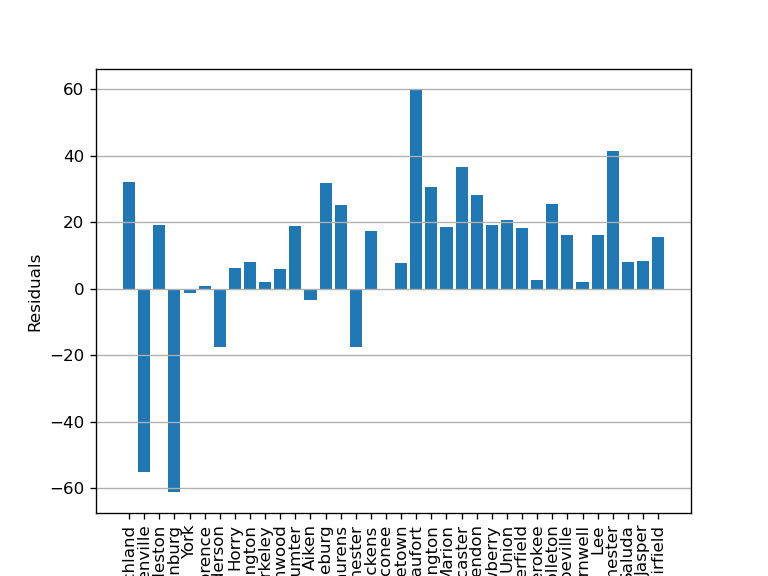
\includegraphics[width=\textwidth]{../../../output/figures/Exploration/resid_plot_County.png}
          \caption{Plot of the residuals for each county, here, the counties are ordered by the number of pleas processed, with the county with the most pleas being first. }
        \end{subfigure}
        \hfill
        \begin{subfigure}[b]{0.45\textwidth}
          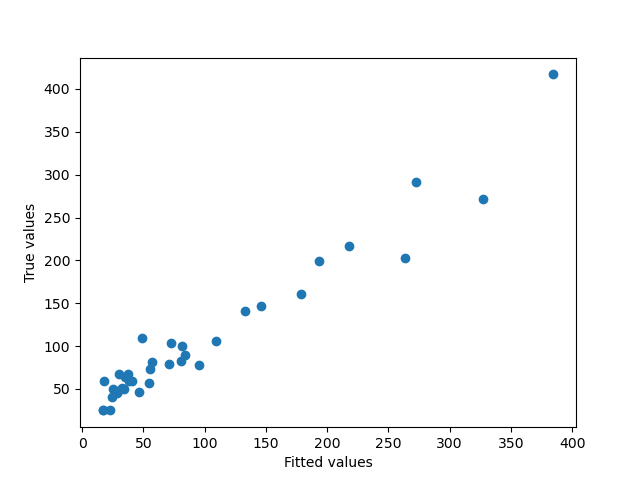
\includegraphics[width=\textwidth]{../../../output/figures/Exploration/true_vs_fitted_County.png}
          \caption{True vs Fitted values for the county model}

        \end{subfigure}
        \label{county-figs}
    \end{figure}

    \begin{table}[H]
      \centering
      \small
      \caption{Lambda Estimates, County Model}
      \label{county-lambda}
      \begin{tabular}{lrrrrrr}
\toprule
{} &  Plea &  Trial &   Days &  TrialDays &  PleaDays &  Lambda \\
County       &       &        &        &            &           &         \\
\midrule
Richland     &  1633 &     25 & 417.00 &     122.07 &    294.93 &    5.54 \\
Greenville   &  1608 &     14 & 272.00 &      68.36 &    203.64 &    7.90 \\
Charleston   &  1329 &     12 & 291.50 &      58.59 &    232.91 &    5.71 \\
Spartanburg  &  1063 &     19 & 202.50 &      92.77 &    109.73 &    9.69 \\
York         &   777 &     19 & 216.50 &      92.77 &    123.73 &    6.28 \\
Florence     &   754 &      5 & 146.50 &      24.41 &    122.09 &    6.18 \\
Anderson     &   655 &     15 & 161.00 &      73.24 &     87.76 &    7.46 \\
Horry        &   655 &     18 & 199.50 &      87.89 &    111.61 &    5.87 \\
Lexington    &   644 &      6 & 141.00 &      29.30 &    111.70 &    5.77 \\
Berkeley     &   382 &      4 &  83.00 &      19.53 &     63.47 &    6.02 \\
Greenwood    &   370 &      5 &  90.00 &      24.41 &     65.59 &    5.64 \\
Sumter       &   353 &      5 & 100.00 &      24.41 &     75.59 &    4.67 \\
Aiken        &   343 &     11 & 105.50 &      53.71 &     51.79 &    6.62 \\
Orangeburg   &   327 &      4 & 104.00 &      19.53 &     84.47 &    3.87 \\
Laurens      &   293 &      2 &  82.00 &       9.77 &     72.23 &    4.06 \\
Dorchester   &   291 &     10 &  78.00 &      48.83 &     29.17 &    9.97 \\
Pickens      &   254 &      3 &  73.00 &      14.65 &     58.35 &    4.35 \\
Oconee       &   230 &      2 &  46.50 &       9.77 &     36.73 &    6.26 \\
Georgetown   &   230 &      7 &  79.00 &      34.18 &     44.82 &    5.13 \\
Beaufort     &   183 &      4 & 109.00 &      19.53 &     89.47 &    2.05 \\
Darlington   &   172 &      2 &  68.00 &       9.77 &     58.23 &    2.95 \\
Marion       &   171 &      1 &  51.00 &       4.88 &     46.12 &    3.71 \\
Lancaster    &   158 &      1 &  67.00 &       4.88 &     62.12 &    2.54 \\
Clarendon    &   158 &      2 &  63.50 &       9.77 &     53.73 &    2.94 \\
Newberry     &   149 &      1 &  48.00 &       4.88 &     43.12 &    3.46 \\
Union        &   147 &      3 &  59.00 &      14.65 &     44.35 &    3.31 \\
Chesterfield &   131 &      4 &  59.00 &      19.53 &     39.47 &    3.32 \\
Cherokee     &   128 &      7 &  57.50 &      34.18 &     23.32 &    5.49 \\
Colleton     &   124 &      1 &  50.50 &       4.88 &     45.62 &    2.72 \\
Abbeville    &   118 &      2 &  45.00 &       9.77 &     35.23 &    3.35 \\
Barnwell     &   113 &      1 &  25.00 &       4.88 &     20.12 &    5.62 \\
Lee          &    91 &      2 &  40.50 &       9.77 &     30.73 &    2.96 \\
Chester      &    79 &      1 &  59.00 &       4.88 &     54.12 &    1.46 \\
Saluda       &    74 &      1 &  25.00 &       4.88 &     20.12 &    3.68 \\
Jasper       &    73 &      1 &  25.00 &       4.88 &     20.12 &    3.63 \\
Fairfield    &    62 &      5 &  50.00 &      24.41 &     25.59 &    2.42 \\
\bottomrule
\end{tabular}

    \end{table}

  \subsection{Judge Model}
    \begin{figure}[H]
      \centering
        \begin{subfigure}[b]{0.45\textwidth}
          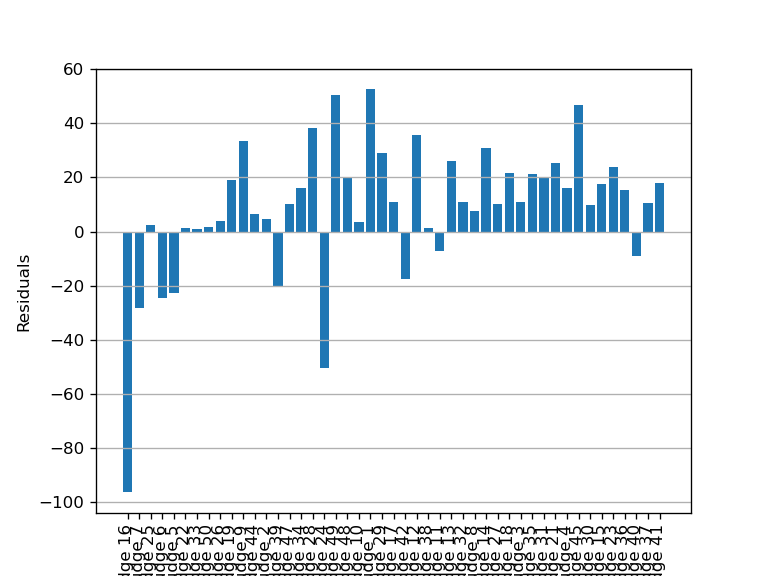
\includegraphics[width=\textwidth]{../../../output/figures/Exploration/resid_plot_JudgeID.png}
          \caption{Plot of the residuals for each Judge, here, the judges are ordered by the number of pleas processed, with the judge with the most pleas being first. }
        \end{subfigure}
        \hfill
        \begin{subfigure}[b]{0.45\textwidth}
          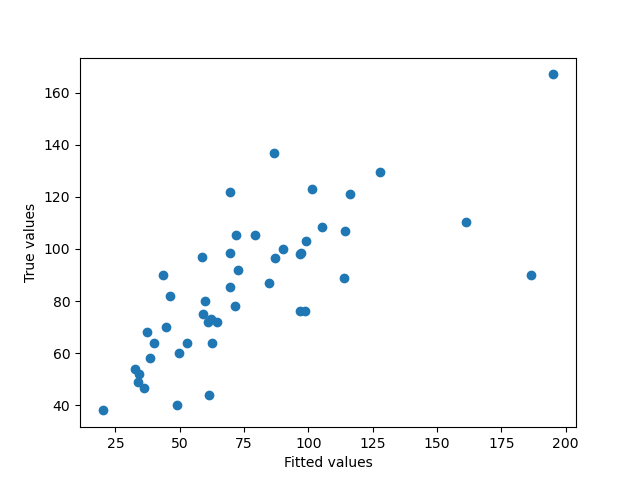
\includegraphics[width=\textwidth]{../../../output/figures/Exploration/true_vs_fitted_JudgeID.png}
          \caption{True vs Fitted values for the Judge model}

        \end{subfigure}
        \label{judge-figs}
    \end{figure}

    \begin{table}[H]
      \centering
      \small
      \caption{Lambda Estimates, Judge Model}
      \label{judge-lambda}
      \begin{tabular}{lrrrrrr}
\toprule
{} &  Plea &  Trial &   Days &  TrialDays &  PleaDays &   Lambda \\
JudgeID  &       &        &        &            &           &          \\
\midrule
Judge 16 &  1041 &      5 &  90.00 &      32.53 &     57.47 &    18.11 \\
Judge 7  &   572 &     17 & 167.00 &     110.59 &     56.41 &    10.14 \\
Judge 25 &   527 &      1 &  87.00 &       6.51 &     80.49 &     6.55 \\
Judge 6  &   505 &      6 &  89.00 &      39.03 &     49.97 &    10.11 \\
Judge 5  &   492 &      4 &  76.00 &      26.02 &     49.98 &     9.84 \\
Judge 22 &   480 &      4 &  98.50 &      26.02 &     72.48 &     6.62 \\
Judge 33 &   479 &      4 &  98.00 &      26.02 &     71.98 &     6.65 \\
Judge 50 &   469 &      9 & 129.50 &      58.55 &     70.95 &     6.61 \\
Judge 26 &   450 &      5 & 103.00 &      32.53 &     70.47 &     6.39 \\
Judge 19 &   404 &      2 &  92.00 &      13.01 &     78.99 &     5.11 \\
Judge 9  &   398 &      2 & 105.50 &      13.01 &     92.49 &     4.30 \\
Judge 44 &   395 &      2 &  78.00 &      13.01 &     64.99 &     6.08 \\
Judge 2  &   390 &      9 & 121.00 &      58.55 &     62.45 &     6.24 \\
Judge 39 &   389 &      6 &  76.00 &      39.03 &     36.97 &    10.52 \\
Judge 47 &   388 &      5 & 100.00 &      32.53 &     67.47 &     5.75 \\
Judge 34 &   355 &      1 &  75.00 &       6.51 &     68.49 &     5.18 \\
Judge 28 &   353 &      1 &  97.00 &       6.51 &     90.49 &     3.90 \\
Judge 24 &   341 &     17 & 110.50 &     110.59 &     -0.09 & -3666.06 \\
Judge 49 &   321 &      6 & 137.00 &      39.03 &     97.97 &     3.28 \\
Judge 48 &   317 &      2 &  80.00 &      13.01 &     66.99 &     4.73 \\
Judge 10 &   315 &      9 & 108.50 &      58.55 &     49.95 &     6.31 \\
Judge 1  &   293 &      4 & 122.00 &      26.02 &     95.98 &     3.05 \\
Judge 29 &   293 &      4 &  98.50 &      26.02 &     72.48 &     4.04 \\
Judge 17 &   288 &      3 &  73.00 &      19.52 &     53.48 &     5.38 \\
Judge 42 &   283 &      3 &  44.00 &      19.52 &     24.48 &    11.56 \\
Judge 12 &   268 &      1 &  82.00 &       6.51 &     75.49 &     3.55 \\
Judge 38 &   247 &      4 &  64.00 &      26.02 &     37.98 &     6.50 \\
Judge 11 &   244 &     12 & 107.00 &      78.07 &     28.93 &     8.43 \\
Judge 13 &   228 &      7 & 105.50 &      45.54 &     59.96 &     3.80 \\
Judge 32 &   226 &      3 &  64.00 &      19.52 &     44.48 &     5.08 \\
Judge 8  &   215 &      5 &  72.00 &      32.53 &     39.47 &     5.45 \\
Judge 14 &   208 &      1 &  68.00 &       6.51 &     61.49 &     3.38 \\
Judge 27 &   204 &      3 &  60.00 &      19.52 &     40.48 &     5.04 \\
Judge 18 &   202 &     11 & 123.00 &      71.56 &     51.44 &     3.93 \\
Judge 3  &   193 &      5 &  72.00 &      32.53 &     39.47 &     4.89 \\
Judge 35 &   176 &      1 &  54.00 &       6.51 &     47.49 &     3.71 \\
Judge 31 &   171 &      2 &  58.00 &      13.01 &     44.99 &     3.80 \\
Judge 21 &   170 &      3 &  70.00 &      19.52 &     50.48 &     3.37 \\
Judge 4  &   162 &      7 &  85.50 &      45.54 &     39.96 &     4.05 \\
Judge 45 &   161 &      3 &  90.00 &      19.52 &     70.48 &     2.28 \\
Judge 30 &   147 &     10 &  96.50 &      65.05 &     31.45 &     4.67 \\
Judge 15 &   144 &      2 &  52.00 &      13.01 &     38.99 &     3.69 \\
Judge 23 &   139 &      3 &  64.00 &      19.52 &     44.48 &     3.12 \\
Judge 36 &   139 &      2 &  49.00 &      13.01 &     35.99 &     3.86 \\
Judge 40 &   112 &      5 &  40.00 &      32.53 &      7.47 &    14.99 \\
Judge 37 &   112 &      3 &  46.50 &      19.52 &     26.98 &     4.15 \\
Judge 41 &    91 &      1 &  38.00 &       6.51 &     31.49 &     2.89 \\
\bottomrule
\end{tabular}

    \end{table}

\section{County-level Analysis}
  The goal of this exercise was to get a better idea of which are the busiest counties.
  I focused only on GS days. So when I say the number of pleas and number of trials, I mean those that
  happened on GS days.
  We have at least three measures of business: the number of pleas, the number of trials, and
  the number of GS days assigned to a county. I ranked the counties according to a measure
  that combined the three measures. To create this measure, I ranked all of the counties according
  to each measure. I then multiplied each county's score in each measure to create an overall measure.
  So, for example, if Richland had the most pleas, then its ranking according to pleas would be 1. If Richland had the second most trials, then its ranking according to trials would be 2. If it had the sixth most GS days, then its ranking according to GS days would be 6. Richland's overall measure would be $1 \cdot 2 \cdot 6 = 12$. This ranking can be seen in table \ref{overall-ranking}. I also created bar charts of the number of pleas, trials, GS days, and the utilization for each county. I calculate the utilization by using the service rate estimates from the county model to calculate the expected number of days it took to process each county's pleas and trials. I then divide the expected number of days by the actual number of assigned days to get the utilization.

  \begin{table}[H]
    \centering
    \small
    \caption{Ranking of Counties by Busyness}
    \label{overall-ranking}
    \begin{tabular}{llrrrr}
\toprule
{} &        County &  Plea &  Trial &   Days &  OverallScore \\
\midrule
1  &      Richland &  1633 &     25 & 417.00 &             1 \\
2  &    Greenville &  1608 &     14 & 272.00 &            36 \\
3  &          York &   777 &     19 & 216.50 &            40 \\
4  &    Charleston &  1329 &     12 & 291.50 &            42 \\
5  &   Spartanburg &  1063 &     19 & 202.50 &            60 \\
6  &         Horry &   655 &     18 & 199.50 &           192 \\
7  &      Anderson &   655 &     15 & 161.00 &           245 \\
8  &      Florence &   754 &      5 & 146.50 &           672 \\
9  &     Lexington &   644 &      6 & 141.00 &           972 \\
10 &         Aiken &   343 &     11 & 105.50 &          1144 \\
11 &        Sumter &   353 &      5 & 100.00 &          2028 \\
12 &     Greenwood &   370 &      5 &  90.00 &          2464 \\
13 &    Dorchester &   291 &     10 &  78.00 &          2592 \\
14 &      Berkeley &   382 &      4 &  83.00 &          3000 \\
15 &    Orangeburg &   327 &      4 & 104.00 &          3024 \\
16 &    Georgetown &   230 &      7 &  79.00 &          3553 \\
17 &      Beaufort &   183 &      4 & 109.00 &          3570 \\
18 &       Laurens &   293 &      2 &  82.00 &          5520 \\
19 &       Pickens &   254 &      3 &  73.00 &          7524 \\
20 &      Cherokee &   128 &      7 &  57.50 &          8990 \\
21 &    Darlington &   172 &      2 &  68.00 &         11500 \\
22 &       Kershaw &   268 &      0 &  68.00 &         14637 \\
23 &  Chesterfield &   131 &      4 &  59.00 &         15390 \\
24 &         Union &   147 &      3 &  59.00 &         15834 \\
25 &     Clarendon &   158 &      2 &  63.50 &         16800 \\
26 &        Oconee &   230 &      2 &  46.50 &         16800 \\
27 &     Lancaster &   158 &      1 &  67.00 &         19448 \\
28 &     Fairfield &    62 &      5 &  50.00 &         20160 \\
29 &      Marlboro &   174 &      0 &  66.50 &         21758 \\
30 &        Marion &   171 &      1 &  51.00 &         23040 \\
31 &  Williamsburg &   156 &      0 &  61.00 &         24975 \\
32 &       Chester &    79 &      1 &  59.00 &         30044 \\
33 &      Newberry &   149 &      1 &  48.00 &         30492 \\
34 &     Abbeville &   118 &      2 &  45.00 &         32076 \\
35 &           Lee &    91 &      2 &  40.50 &         34632 \\
36 &      Colleton &   124 &      1 &  50.50 &         34720 \\
37 &        Saluda &    74 &      1 &  25.00 &         46740 \\
38 &        Jasper &    73 &      1 &  25.00 &         48360 \\
39 &     Edgefield &   116 &      0 &  34.00 &         49096 \\
40 &      Barnwell &   113 &      1 &  25.00 &         50400 \\
41 &        Dillon &    74 &      0 &  48.00 &         60996 \\
42 &       Bamberg &    70 &      0 &  22.67 &         70520 \\
43 &     McCormick &    47 &      0 &  23.00 &         75852 \\
44 &     Allendale &     8 &      0 &  14.00 &         82524 \\
45 &       Hampton &    33 &      0 &  19.00 &         87120 \\
46 &       Calhoun &    27 &      0 &  14.00 &         89100 \\
\bottomrule
\end{tabular}

  \end{table}

  \subsection{Overall Figures}
   In figure \ref{fig-county}, the counties are ordered according to the overall ranking described in the previous section.

    \begin{figure}[H]
      \centering
        \begin{subfigure}[b]{0.45\textwidth}
          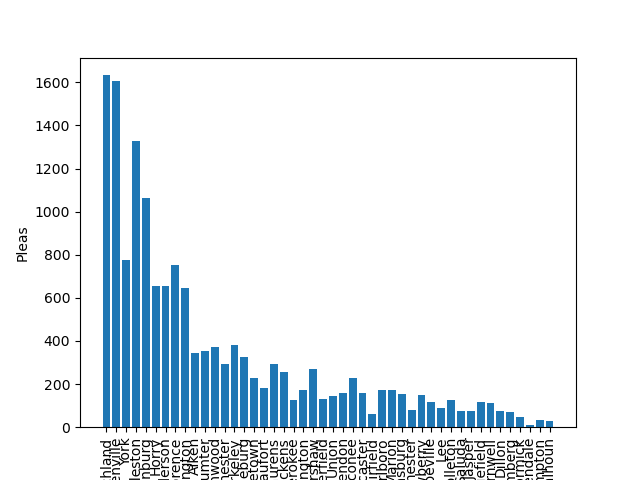
\includegraphics[width=\textwidth]{../../../output/figures/Exploration/county_pleas.png}
          \caption{Pleas}
        \end{subfigure}
        \hfill
        \begin{subfigure}[b]{0.45\textwidth}
          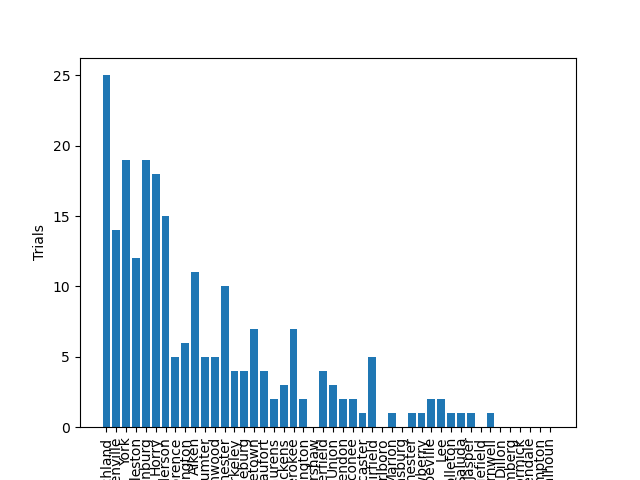
\includegraphics[width=\textwidth]{../../../output/figures/Exploration/county_trials.png}
          \caption{Trials}

        \end{subfigure}
        %\hfill
        \begin{subfigure}[b]{0.45\textwidth}

          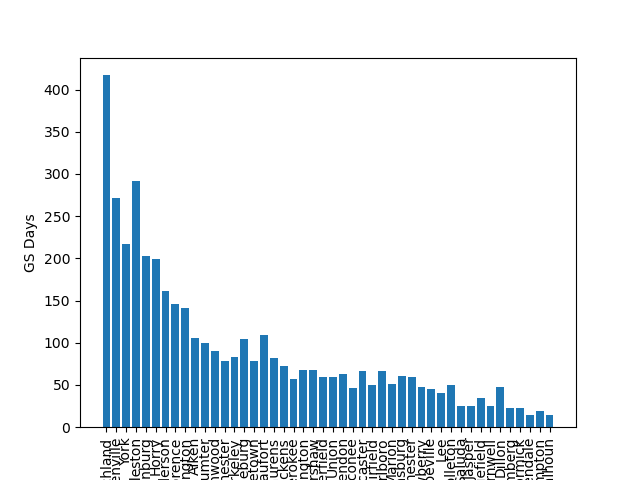
\includegraphics[width=\textwidth]{../../../output/figures/Exploration/county_days.png}
          \caption{GS Days}

        \end{subfigure}
        \hfill
        \begin{subfigure}[b]{0.45\textwidth}

          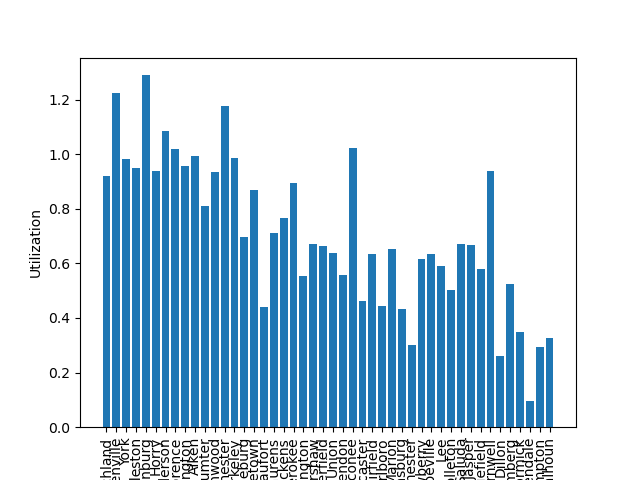
\includegraphics[width=\textwidth]{../../../output/figures/Exploration/county_utilization.png}
          \caption{Utilization}

        \end{subfigure}
        \caption{Number of Pleas, Trials, GS days, and utilization for each county.}
        \label{fig-county}
    \end{figure}

  \subsection{CDF table}
    The purpose of this section is to get a better sense of what share of the overall action happens
    in the 'busy' counties. In table \ref{cdf-table}, the columns PleaShare, TrialShare, and GSShare
    contain the cumulative share of all pleas, trials, and GS days accounted for by the counties up to that row. So, for example, in the 10th row, if the value of PleaShare is 0.5, that means that the top
    10 counties account for $50\%$ of all pleas. Similarly, if in the 15th row the value of Trial share is 0.9, that means that the top 15 counties account for $90\%$ of all trials. GS share refers to the share of all GS days assigned. The counties in table \ref{cdf-table} are ranked using the measure described in the beginning of the section.

    \begin{table}[H]
      \centering
      \small
      \caption{CDF table}
      \label{cdf-table}
      \begin{tabular}{llrrrrrrr}
\toprule
{} &        County &  Plea &  Trial &   Days &  OverallScore &  PleaShare &  TrialShare &  GSDayShare \\
\midrule
1  &      Richland &  1633 &     25 & 417.00 &             1 &       0.11 &        0.11 &        0.10 \\
2  &    Greenville &  1608 &     14 & 272.00 &            36 &       0.21 &        0.17 &        0.17 \\
3  &          York &   777 &     19 & 216.50 &            40 &       0.26 &        0.26 &        0.22 \\
4  &    Charleston &  1329 &     12 & 291.50 &            42 &       0.35 &        0.31 &        0.29 \\
5  &   Spartanburg &  1063 &     19 & 202.50 &            60 &       0.42 &        0.40 &        0.34 \\
6  &         Horry &   655 &     18 & 199.50 &           192 &       0.46 &        0.48 &        0.38 \\
7  &      Anderson &   655 &     15 & 161.00 &           245 &       0.50 &        0.54 &        0.42 \\
8  &      Florence &   754 &      5 & 146.50 &           672 &       0.55 &        0.56 &        0.46 \\
9  &     Lexington &   644 &      6 & 141.00 &           972 &       0.60 &        0.59 &        0.49 \\
10 &         Aiken &   343 &     11 & 105.50 &          1144 &       0.62 &        0.64 &        0.52 \\
11 &        Sumter &   353 &      5 & 100.00 &          2028 &       0.64 &        0.66 &        0.54 \\
12 &     Greenwood &   370 &      5 &  90.00 &          2464 &       0.67 &        0.68 &        0.56 \\
13 &    Dorchester &   291 &     10 &  78.00 &          2592 &       0.68 &        0.73 &        0.58 \\
14 &      Berkeley &   382 &      4 &  83.00 &          3000 &       0.71 &        0.75 &        0.60 \\
15 &    Orangeburg &   327 &      4 & 104.00 &          3024 &       0.73 &        0.76 &        0.63 \\
16 &    Georgetown &   230 &      7 &  79.00 &          3553 &       0.75 &        0.80 &        0.65 \\
17 &      Beaufort &   183 &      4 & 109.00 &          3570 &       0.76 &        0.81 &        0.67 \\
18 &       Laurens &   293 &      2 &  82.00 &          5520 &       0.78 &        0.82 &        0.69 \\
19 &       Pickens &   254 &      3 &  73.00 &          7524 &       0.79 &        0.84 &        0.71 \\
20 &      Cherokee &   128 &      7 &  57.50 &          8990 &       0.80 &        0.87 &        0.72 \\
21 &    Darlington &   172 &      2 &  68.00 &         11500 &       0.81 &        0.88 &        0.74 \\
22 &       Kershaw &   268 &      0 &  68.00 &         14637 &       0.83 &        0.88 &        0.76 \\
23 &  Chesterfield &   131 &      4 &  59.00 &         15390 &       0.84 &        0.89 &        0.77 \\
24 &         Union &   147 &      3 &  59.00 &         15834 &       0.85 &        0.91 &        0.78 \\
25 &     Clarendon &   158 &      2 &  63.50 &         16800 &       0.86 &        0.92 &        0.80 \\
26 &        Oconee &   230 &      2 &  46.50 &         16800 &       0.87 &        0.92 &        0.81 \\
27 &     Lancaster &   158 &      1 &  67.00 &         19448 &       0.88 &        0.93 &        0.83 \\
28 &     Fairfield &    62 &      5 &  50.00 &         20160 &       0.89 &        0.95 &        0.84 \\
29 &      Marlboro &   174 &      0 &  66.50 &         21758 &       0.90 &        0.95 &        0.85 \\
30 &        Marion &   171 &      1 &  51.00 &         23040 &       0.91 &        0.96 &        0.87 \\
31 &  Williamsburg &   156 &      0 &  61.00 &         24975 &       0.92 &        0.96 &        0.88 \\
32 &       Chester &    79 &      1 &  59.00 &         30044 &       0.93 &        0.96 &        0.90 \\
33 &      Newberry &   149 &      1 &  48.00 &         30492 &       0.94 &        0.96 &        0.91 \\
34 &     Abbeville &   118 &      2 &  45.00 &         32076 &       0.94 &        0.97 &        0.92 \\
35 &           Lee &    91 &      2 &  40.50 &         34632 &       0.95 &        0.98 &        0.93 \\
36 &      Colleton &   124 &      1 &  50.50 &         34720 &       0.96 &        0.99 &        0.94 \\
37 &        Saluda &    74 &      1 &  25.00 &         46740 &       0.96 &        0.99 &        0.95 \\
38 &        Jasper &    73 &      1 &  25.00 &         48360 &       0.97 &        1.00 &        0.95 \\
39 &     Edgefield &   116 &      0 &  34.00 &         49096 &       0.98 &        1.00 &        0.96 \\
40 &      Barnwell &   113 &      1 &  25.00 &         50400 &       0.98 &        1.00 &        0.97 \\
41 &        Dillon &    74 &      0 &  48.00 &         60996 &       0.99 &        1.00 &        0.98 \\
42 &       Bamberg &    70 &      0 &  22.67 &         70520 &       0.99 &        1.00 &        0.98 \\
43 &     McCormick &    47 &      0 &  23.00 &         75852 &       1.00 &        1.00 &        0.99 \\
44 &     Allendale &     8 &      0 &  14.00 &         82524 &       1.00 &        1.00 &        0.99 \\
45 &       Hampton &    33 &      0 &  19.00 &         87120 &       1.00 &        1.00 &        1.00 \\
46 &       Calhoun &    27 &      0 &  14.00 &         89100 &       1.00 &        1.00 &        1.00 \\
\bottomrule
\end{tabular}

    \end{table}

  \subsection{Comparing Busy and Idle Counties}
    The purpose of this section is to further investigate how 'busy' counties are different from 'idle'
    counties. To do this, I split the counties into above median and below median in terms of business.
    Here, business is measured according to the measure described in the beginning of the section.

    \begin{figure}[H]
      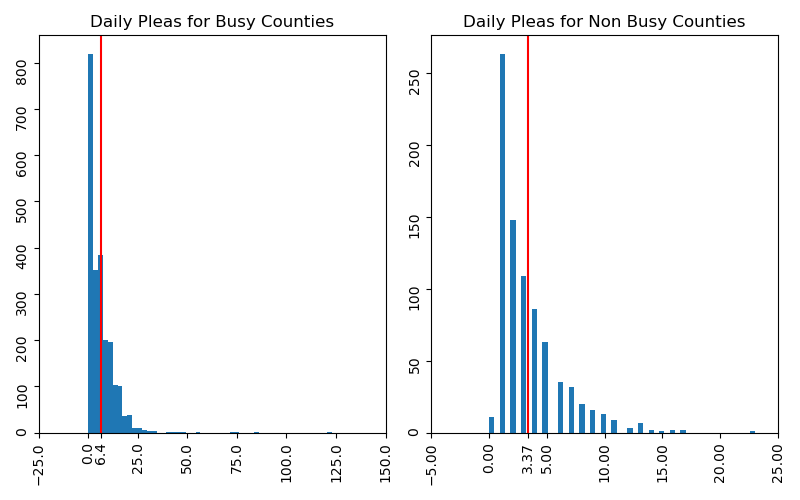
\includegraphics[width=0.9\textwidth]{../../../output/figures/Exploration/busy_vs_idle_plea_hists.png}
      \caption{Histogram of pleas processed per day}
      \label{plea-hist}
    \end{figure}

    \begin{figure}[H]
      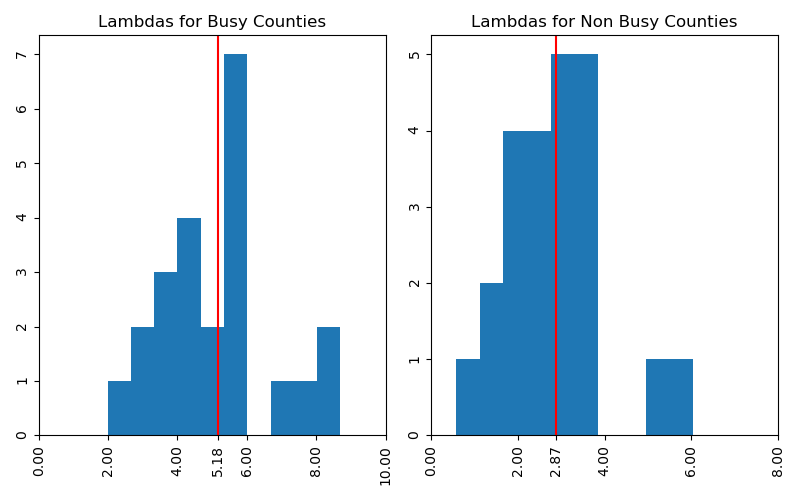
\includegraphics[width=0.9\textwidth]{../../../output/figures/Exploration/lambda_hists.png}
      \caption{Histogram of estimated lambda}
      \label{lambda-hist}
    \end{figure}

\section{Clean Day Analysis}
  The purpose of this section is to better understand clean days.
  In our previous meeting, we wanted to know what exactly was driving the large difference in average number of pleas between clean days and GS days. As a reminder, the average number of pleas for GS days was around 5, and the average number of pleas for clean days was 14. It turns out that this
  was driven by our restriction that clean days have more than 10 pleas.

  To better understand clean days, we first
  list our clean day restrictions and study how each of them affects the average number of
  pleas processed per day. Then, we examine how the clean days are distributed across
  judges and counties.

  \subsection{Clean Day Restrictions}
    \begin{itemize}
      \item Exclude all days in which there is a conflict between the sentencing data and the calendar data.
      \item Exclude all non-GS days.
      \item Exclude all days in which a judge sentenced in more than one county.
      \item Exclude all days in which a judge was assigned to more than one county.
      \item Exclude all days in which a judge sentenced fewer than 10 events.
    \end{itemize}

    \begin{table}[H]
      \centering
      \small
      \caption{Clean Day Restrictions. This table describes how the average number of pleas processed per day evolves as restrictions are added.}
      \label{clean-day-rest}
      \begin{tabular}{lr}
\toprule
                     Restriction &  Average Pleas Per Day \\
\midrule
                            None &                   5.04 \\
             No conflicting days &                   4.89 \\
                    Only GS days &                   4.86 \\
            No mutli-county days &                   4.86 \\
        No mutli-assignment days &                   4.87 \\
No days with less than 10 events &                  14.57 \\
\bottomrule
\end{tabular}

    \end{table}

  \subsection{Distribution of Clean Days Across Counties}
    \begin{figure}[H]
      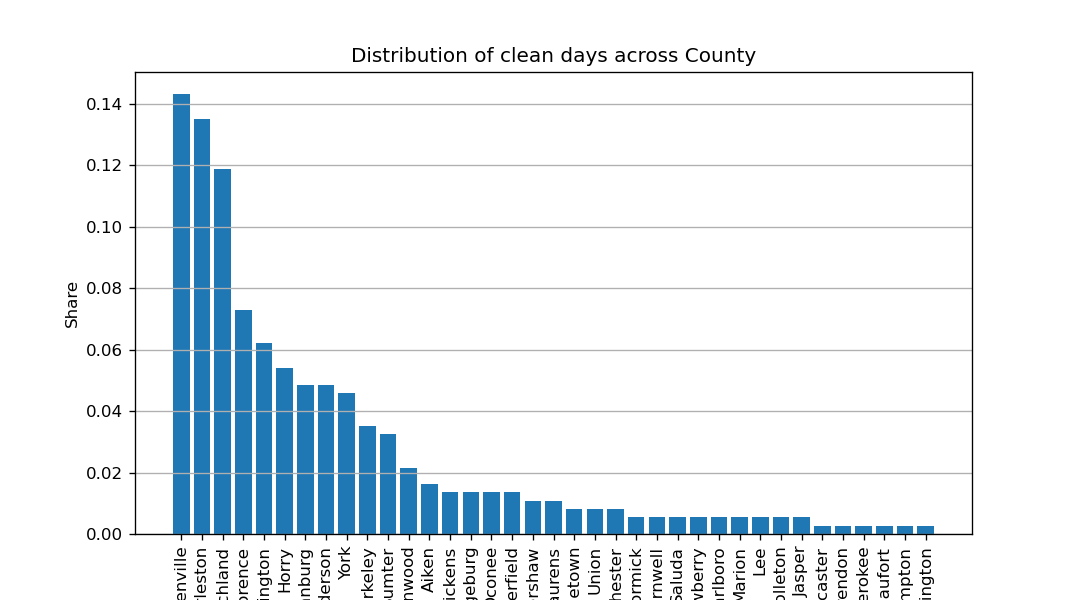
\includegraphics[width=0.9\textwidth]{../../../output/figures/Exploration/clean_day_dist_County.png}
      \caption{Distribution of clean days across counties}
    \end{figure}

  \subsection{Distribution of Clean Days Across Judges}
    \begin{figure}[H]
      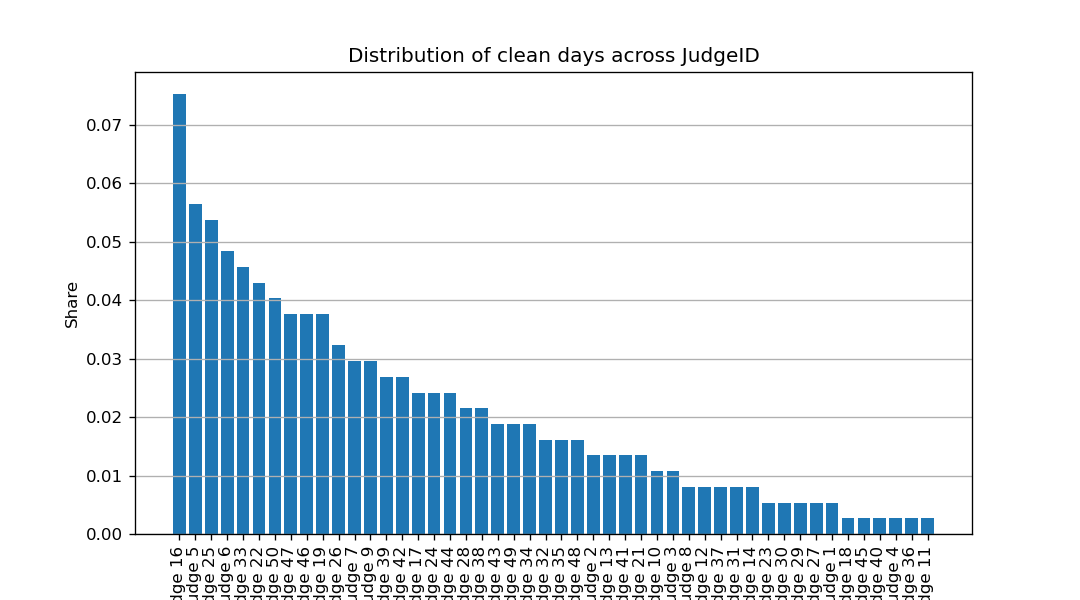
\includegraphics[width=0.9\textwidth]{../../../output/figures/Exploration/clean_day_dist_JudgeID.png}
      \caption{Distribution of clean days across counties}
    \end{figure}

\end{document}
